\chapter{Spring Data JPA}

\fcolorbox{black}[HTML]{E9F0E9}{\parbox{\textwidth}{%
\noindent \textbf{Learning goals}\\
The junior-colleague
\begin{enumerate}[nolistsep]
\item can describe the concept of ORM.
\item can explain what JPA is, and what it’s not.
\item can denominate different JPA providers.
\item can describe what a persistence unit is.
\item can explain the fundamental interfaces of JPA.
\item can explain what the persistence context is.
\item can implement entity classes.
\item can describe the entity objects’ lifecycle.
\item can implement different types of relationships between entity classes.
\item can implement CRUD operations.
\item can implement queries.
\item can implement named queries.
\item can explain, identify and solve the N + 1 query problem.
\end{enumerate}}}

  
\section{What is ORM?}

Object-Relational Mapping (ORM) is a technique that lets you query and manipulate data from a relational database using an object-oriented programming language.

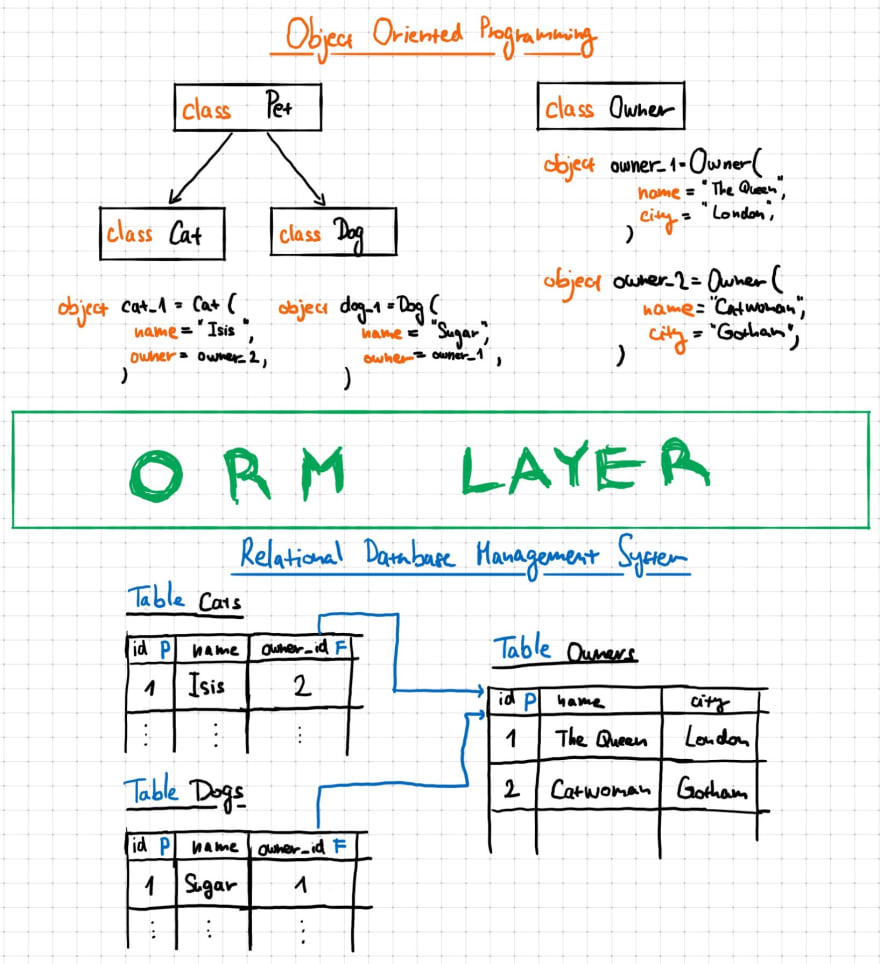
\includegraphics[width=\textwidth]{./images/chapter6/orm}


\section{What is JPA?}

The Java Persistence API (JPA; recently renamed to Jakarta Persistence API) is a specification that defines how to persist data in Java applications. JPA mainly focuses on the ORM layer and managing persistent objects.

JPA is a specification which means JPA consists of implementation guidelines for the Java ORM layer and the syntax. The specification only comes with interfaces, no actual implementation.  A reference implementation can be provided but other companies can create and distribute their own implementation of the specification.

\frame{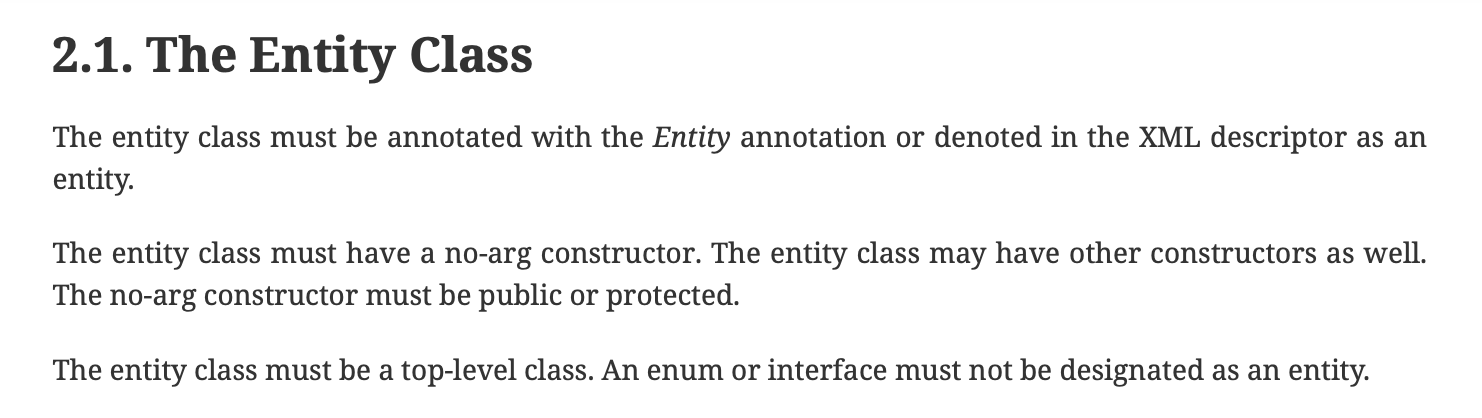
\includegraphics[width=\textwidth]{./images/chapter6/entity_class_specification}}

For our exercises and projects we will use Hibernate as the actual implementation of de JPA specification \footnote{\url{https://hibernate.org/ and https://hibernate.org/orm/}}.  

Spring Data JPA adds a layer on top of JPA. It uses all the features defined by the JPA specification, but adds no-code implementation of the repository pattern and the creation of database queries from method names.

The JpaRepository interface is an extension of CrudRepository.
JpaRepository extends PagingAndSortingRepository which in turn extends CrudRepository.

Their main functions are:

\begin{itemize}
\item CrudRepository mainly provides CRUD functions.
\item PagingAndSortingRepository provides methods to do pagination and sorting records.
\item JpaRepository provides some JPA-related methods such as flushing the persistence context and deleting records in a batch.
\end{itemize}


\section{Datasource}

In Spring Boot a DataSource-object is the preferred means of getting a connection to a database.
The interface jakarta.sql.DataSource is implemented by the database driver vendor. 

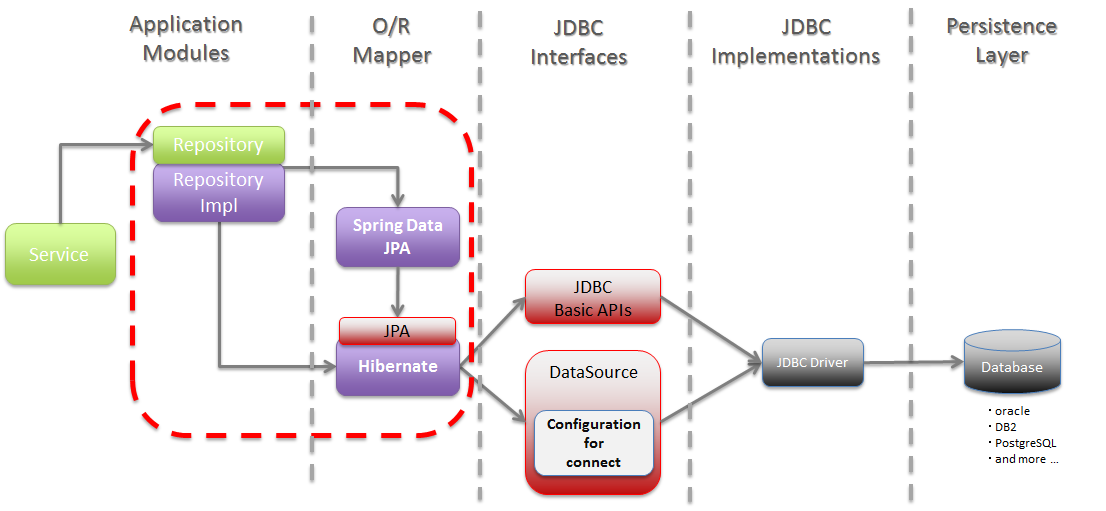
\includegraphics[width=\textwidth]{./images/chapter-jpa/springdatajpa}

The datasource can be specified in the application.properties file.
Here are some common database properties:

\begin{tabular}{|l|p{8cm}|}
\hline
spring.datasource.url & JDBC URL of the database.\\
spring.datasource.username & Login username of the database.\\
spring.datasource.password & Login password of the database.\\
spring.jpa.show-sql & Whether to enable logging of SQL statements. Default: false\\
spring.jpa.hibernate.ddl-auto & Possible values: none (production), create, create-drop, validate and update. \footnote{\url{https://stackoverflow.com/questions/42135114/how-does-spring-jpa-hibernate-ddl-auto-property-exactly-work-in-spring}}\\
\hline
\end{tabular}

Alternatively, the data source configuration can be programmatically.

The appropriate JDBC driver for your database must be included in your project. This is achieved by declaring the driver as a dependency in your project's Maven configuration file, pom.xml. The dependency ensures that the JDBC driver is available during runtime, allowing Spring Data JPA to establish and manage database connections.

Here is an example of how to include a JDBC driver for MySQL in your pom.xml file:

\begin{lstlisting}
<dependency>
<groupId>com.mysql</groupId>
<artifactId>mysql-connector-j</artifactId>
<scope>runtime</scope>
</dependency>
\end{lstlisting}

This configuration snippet includes the MySQL JDBC driver, mysql-connector-j.

Similarly,  to connect to a PostgreSQL database, you would use the PostgreSQL JDBC driver as shown below:

\begin{lstlisting}
<dependency>
<groupId>org.postgresql</groupId>
<artifactId>postgresql</artifactId>
<scope>runtime</scope>
</dependency>
\end{lstlisting}

Adjusting the driver version in your pom.xml may be necessary as you upgrade your database server or migrate to a newer version of Spring Data JPA.


\section{The Entity class}

\begin{lstlisting}[frame=single,language=java]
import jakarta.persistence.Entity;
import jakarta.persistence.Table;
import jakarta.persistence.Column;
import jakarta.persistence.Id;
import jakarta.persistence.GeneratedValue;
import jakarta.persistence.GenerationType;
import jakarta.persistence.Embedded;
import jakarta.persistence.Embeddable;

@Entity
@Table(name = "events")
public class Event {

    @Id
    @GeneratedValue(strategy = GenerationType.IDENTITY)
    private Long id;

    @Column(name = "name", nullable = false,  length = 200)
    private String title;

    @Embedded
    private EventDetails details;

    // Constructors, getters, and setters
}

@Embeddable
class EventDetails {
    private LocalDate date;
    @Column(length = 512)
    private String location;

    // Constructors, getters, and setters
}
\end{lstlisting}

A JPA entity class is a POJO (Plain Old Java Object) class  that is annotated as having the ability to represent objects in the database.
The \textbf{@Entity} annotation is used to declare that a class is an entity, so JPA will manage it and map it to a database table.

\textbf{@Table} specifies the table in the database with which the entity is mapped.

The \textbf{@Id} annotation marks a field as a primary key field.

The \textbf{@GeneratedValue} annotation is used to configure the primary key generation strategy for an entity. This annotation is usually combined with @Id to specify that the persistence provider should automatically generate a unique identifier for the entity objects. There are several strategies defined in the GenerationType enumeration that can be used with @GeneratedValue. Here's an overview:

\begin{itemize}
\item \textbf{GenerationType.AUTO}

This is the default strategy and the persistence provider will choose the generation strategy based on the specific database capabilities and dialect. 

\item \textbf{GenerationType.IDENTITY}

Indicates that the persistence provider must assign primary keys using the database identity column. This is typically supported by SQL databases with an auto-increment column.

\item \textbf{GenerationType.SEQUENCE}

Specifies that the primary key values will be generated using a database sequence. This is a special database object that generates numbers in sequential order. Not all databases support sequences.
This strategy is useful for databases supporting sequences, like Oracle, PostgreSQL, etc. It's beneficial for high-volume applications due to better performance compared to IDENTITY, as the sequence generation can be more efficiently managed.

\item \textbf{GenerationType.TABLE}

Uses a database table to simulate a sequence. This strategy uses a table to hold the next id incrementally. It's a portable solution but not as efficient as using database-specific features like sequences or identity columns.
\end{itemize}

The \textbf{@Column} annotation is used to specify the details of the column to which a field or property will be mapped. You can use column annotation with the following most commonly used attributes:
\begin{itemize}
\item \textbf{name}: specify the name of the column.
\item \textbf{length}: specify the size of thee column, particularly for a String value.
\item \textbf{nullable}: mark the column to be NOT NULL when the database schema is generated.
\item \textbf{unique}: mark the column to contain only unique values.
\end{itemize}


The \textbf{@Embeddable} annotation marks a class to be embedded within another entity.
In this example,  the EventDetails does not need its own table; instead, its properties are incorporated into the table of the entity that embeds it.

The annotation \textbf{@Embedded}  is used to denote a class whose instances are stored as an intrinsic part of an owning entity.
 All the fields of EventDetails class are embedded within the events table, avoiding the need for a separate table.


\section{Entity lifecycle}

The EntityManager is a core interface of JPA.  An instance of EntityManager is used to create and remove  entity instances, to find entities by their primary key,  and to query over entities.  In fact,  an instance of the EntityManager is used to interact with the persistence context. 

The persistence context is one of the main concepts in JPA.
It is a set of all entity object that you are currently using or used recently. You can think of the persistence context as some kind of first-level cache. Each entity object in the persistence context represents a record in the database.
The persistence context manages these entity objects and their lifecycle. Each entity object has one of 4 states: new, managed, removed, and detached.

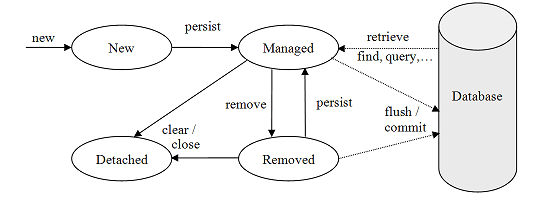
\includegraphics[width=\textwidth]{./images/chapter6/entity_states}

A newly instantiated entity object is in state \textbf{new} or \textbf{transient}. The entity object hasn't been persisted yet, so there's no database record yet. The persistence context does not know about the entity object yet. 

All entity objects that attached to the persistence context are in the lifecycle state \textbf{managed}. An entity object becomes managed when it is persisted to the database. Entity object retrieved from the database are also in the managed state.
If a managed entity object is modified (updated) within an active transaction, the change is detected by the persistence context and passed on to the database.

When a managed entity is removed within an active transaction, the state changes from managed to removed, and the record is physically deleted from the database (when the transaction commits).

An entity gets detached when it is no longer managed by the persistence context but still represents a record in the database.
Detached objects are limited in functionality.

 
Programmatically we need to use the entitymanager to change the state of the entity object in the persistence context which results in changes or updates in our database. 

When using Spring Data JPA you don't have to implement the interaction with the entitymanager. When you create a Repository, the SimpleJpaRepository class provided by Spring Data JPA provides the default implementation. SimpleJpaRepository class internally uses JPA entitymanager.

\begin{oefening}
Open the class SimpleJpaRepository and take a look at its implementation (e.g. save()-method).
\end{oefening}


\section{Relationships}

\subsection{OneToOne relationship}

A OneToOne relationship in JPA is used when one entity instance is associated with exactly one instance of another entity.  In this example a user has exactly one passport.

In a \textbf{uni-directional} OneToOne relationship, only one side of the relationship maintains knowledge of the other side’s existence. Consider a scenario where each Person has exactly one Passport. The Person entity holds a reference to the Passport, but the Passport does not hold any reference to the Person.

\begin{lstlisting}
@Entity
public class Person {
    @Id
    @GeneratedValue(strategy = GenerationType.IDENTITY)
    private Long id;
    
    @OneToOne(cascade = CascadeType.ALL)
    @JoinColumn(name = "passport_id", referencedColumnName = "id")
    private Passport passport;

    // Standard getters and setters
}

@Entity
public class Passport {
    @Id
    @GeneratedValue(strategy = GenerationType.IDENTITY)
    private Long id;
    
    private String number;

    // Standard getters and setters
}
\end{lstlisting}

In this example, the Person entity contains a Passport field annotated with @OneToOne. The @JoinColumn annotation specifies the column in the Person table that joins to the primary key of the Passport entity.

The concept of \"cascade types\" defines how persistence operations such as save, delete, and update performed on one entity should be propagated (or cascaded) to its associated entity. 

When using the @OneToOne annotation in JPA, you can specify a cascade type to automate the persistence lifecycle management of the associated entity. Here are the most common cascade types used in JPA:

\begin{itemize}
\item \textbf{CascadeType.PERSIST}: When persisting an entity, also persist the associated entity.  For example, when saving a Person object, also save its associated Passport.

\item \textbf{CascadeType.MERGE}: When merging the state of an entity into the current persistence context, also merge the entity held in this field.

\item \textbf{CascadeType.REMOVE}: When deleting an entity, also delete the associated entity. This is particularly useful when the associated entity no longer makes sense to exist independently.

\item \textbf{CascadeType.REFRESH}: When refreshing an entity, also refresh the entities held in this field. This means reloading the content of the associated entity from the database, which can be useful if the database might be changed by other processes.

\item \textbf{CascadeType.DETACH}: When an entity is detached from the persistence context, also detach the entities held in this field.

\item \textbf{CascadeType.ALL}: A convenience that cascades all the above operations (PERSIST, MERGE, REMOVE, REFRESH, DETACH). Using CascadeType.ALL is common for @OneToOne and @OneToMany associations.
\end{itemize}

In a \textbf{bi-directional} OneToOne relationship, both entities are aware of each other. This relationship allows navigation from either side. Using the same example as above, both the Person and Passport entities can have references to each other.

\begin{lstlisting}
@Entity
public class Person {
    @Id
    @GeneratedValue(strategy = GenerationType.IDENTITY)
    private Long id;

    @OneToOne(mappedBy = "person", cascade = CascadeType.ALL)
    private Passport passport;

    // Standard getters and setters
}

@Entity
public class Passport {
    @Id
    @GeneratedValue(strategy = GenerationType.IDENTITY)
    private Long id;

    private String number;

    @OneToOne
    @JoinColumn(name = "person_id")
    private Person person;

    // Standard getters and setters
}
\end{lstlisting}

In this bi-directional setup, the Person entity uses the mappedBy attribute in the @OneToOne annotation to indicate that the Person is not the owner of the relationship and that the Passport entity contains the foreign key.

\subsection{ManyToOne relationship}

A ManyToOne relationship in JPA is commonly used when one entity is related to multiple instances of another entity. For instance, in a blog system, many posts may belong to one category. Below, I will provide examples of both uni-directional and bi-directional ManyToOne relationships, suitable for inclusion in a student's textbook or educational material on Spring Data JPA.

Uni-directional ManyToOne Relationship
In a uni-directional ManyToOne relationship, only the 'many' side of the relationship is aware of the 'one' side. This setup is often seen when the 'one' side doesn't need to directly access the 'many' side.

Example: Books and Authors
Suppose each book can have one author, but each author can write many books. Here, the relationship from books to authors is a typical example of a uni-directional ManyToOne relationship.

Entity Definition
java
Copy code
@Entity
public class Book {
    @Id
    @GeneratedValue(strategy = GenerationType.IDENTITY)
    private Long id;

    private String title;

    @ManyToOne
    @JoinColumn(name = "author_id", nullable = false)
    private Author author;

    // Standard getters and setters
}

@Entity
public class Author {
    @Id
    @GeneratedValue(strategy = GenerationType.IDENTITY)
    private Long id;

    private String name;

    // Standard getters and setters, no reference back to Book
}
In this model, each Book entity holds a reference to its Author, which is annotated with @ManyToOne. The @JoinColumn annotation specifies the foreign key column in the Book table that links to the Author.

Repository Configuration
Repositories for each entity can be defined as follows:

java
Copy code
public interface BookRepository extends JpaRepository<Book, Long> {
}

public interface AuthorRepository extends JpaRepository<Author, Long> {
}
Bi-directional ManyToOne Relationship
In a bi-directional relationship, both sides of the relationship are aware of each other. This is useful when you want to navigate the relationship from either side.

Example: Books and Authors Continued
Expanding on the previous example, suppose now we want authors to also be aware of the books they've written.

Entity Definition
java
Copy code
@Entity
public class Book {
    @Id
    @GeneratedValue(strategy = GenerationType.IDENTITY)
    private Long id;

    private String title;

    @ManyToOne
    @JoinColumn(name = "author_id", nullable = false)
    private Author author;

    // Standard getters and setters
}

@Entity
public class Author {
    @Id
    @GeneratedValue(strategy = GenerationType.IDENTITY)
    private Long id;

    private String name;

    @OneToMany(mappedBy = "author")
    private Set<Book> books = new HashSet<>();

    // Standard getters and setters
}
In this bi-directional setup, the Author class includes a Set<Book> to hold the collection of books. The @OneToMany annotation in Author uses the mappedBy attribute to indicate that the Author entity is not the owner of the relationship and that the Book entity contains the foreign key.

\subsection{ManyToMany relationship}


A ManyToMany relationship is used when multiple instances of one entity are associated with multiple instances of another entity. Using the example of books and authors, a ManyToMany relationship would be appropriate if each book could have multiple authors and each author could write multiple books. 

In a uni-directional ManyToMany relationship, only one entity maintains the relationship information.

Imagine a scenario where each book can have multiple authors, but we are only interested in navigating from books to authors and not the other way around.

\begin{lstlisting}
@Entity
public class Book {
    @Id
    @GeneratedValue(strategy = GenerationType.IDENTITY)
    private Long id;

    private String title;

    @ManyToMany
    @JoinTable(
        name = "book_author",
        joinColumns = @JoinColumn(name = "book_id"),
        inverseJoinColumns = @JoinColumn(name = "author_id")
    )
    private Set<Author> authors = new HashSet<>();

    // Standard getters and setters
}

@Entity
public class Author {
    @Id
    @GeneratedValue(strategy = GenerationType.IDENTITY)
    private Long id;

    private String name;

    // Standard getters and setters, no reference back to Books
}
\end{lstlisting}
In this example, the Book entity defines a ManyToMany relationship to the Author entity. The @JoinTable annotation specifies the table that maps books to authors, including columns for each foreign key.


In a bi-directional ManyToMany relationship, both entities are aware of each other, and navigation is possible from either side.

This time, both books and authors are aware of each other and can navigate the relationship.

\begin{lstlisting}
@Entity
public class Book {
    @Id
    @GeneratedValue(strategy = GenerationType.IDENTITY)
    private Long id;

    private String title;

    @ManyToMany
    @JoinTable(
        name = "book_author",
        joinColumns = @JoinColumn(name = "book_id"),
        inverseJoinColumns = @JoinColumn(name = "author_id")
    )
    private Set<Author> authors = new HashSet<>();

    // Standard getters and setters
}

@Entity
public class Author {
    @Id
    @GeneratedValue(strategy = GenerationType.IDENTITY)
    private Long id;

    private String name;

    @ManyToMany(mappedBy = "authors")
    private Set<Book> books = new HashSet<>();

    // Standard getters and setters
}
\end{lstlisting}

In the bi-directional arrangement, the Author entity includes a Set<Book> to hold the collection of books. The mappedBy attribute indicates that the Author is not the owner of the relationship, and the mapping details are managed by the Book entity.

\section{Fetching strategy}

JPA provides two main fetching strategies to control how related entities are loaded from the database:

\begin{itemize}
\item \textbf{Eager Fetching}: With eager fetching, related entities are loaded immediately with the main entity, whether they are accessed in the application or not. This can lead to performance issues if the relationships involve large sets of data. Eager fetching is often used when the data sets are small or always used together with the main entity.

Lazy Fetching: Lazy fetching loads the related entities only when they are explicitly accessed in the application. This can improve performance by reducing the initial load time and the amount of memory consumed. However, it requires careful management of the persistence context to avoid LazyInitializationException.

java
Copy code
@ManyToMany(fetch = FetchType.LAZY)
private Set<Author> authors = new HashSet<>();
In the case of ManyToMany relationships, the default fetching strategy is lazy because eager fetching can result in very large numbers of joins and thus severe performance degradation.

Understanding and choosing the right fetching strategy based on the specific use case and data access patterns is crucial for developing efficient, scalable applications.

\section{Queries}

Basic CRUD queries are in Spring Data JPA available in the repositories. But there are multiple ways of creating custom queries in a Spring boot application. Let's discuss the different
types of queries.

\subsection{Query methods}

Spring Data JPA can create queries based on method names. You can use keywords like \textit{findBy}, \textit{findAllBy},
\textit{findBy...And...}, ...

An overview of the keywords can be found in spring documentation \url{https://docs.spring.io/spring-data/jpa/reference/jpa/query-methods.html}.

\begin{lstlisting}
public interface ProductRepository extends JpaRepository<Product, Long> {
    // Query method with parameters for finding products by name and price
    List<Product> findByNameAndPrice(String name, double price);
}
\end{lstlisting}

\subsection{JPQL queries}

JPQL, or Java Persistence Query Language, is a query language designed to abstract database details from the developer, allowing queries to be written based on entity model classes rather than on database tables.


\begin{lstlisting}
public interface UserRepository extends JpaRepository<User, Long> {
  @Query("SELECT u FROM User u WHERE u.age >= :minAge")
  List<User> findByAgeGreaterThan(@Param("minAge") int minAge);
}
\end{lstlisting}

\subsection{Native SQL queries}

\begin{lstlisting}

\end{lstlisting}


\section{Unit testing a repository}

Spring Data JPA offers an annotation @DataJpaTest which makes repository testing possible with a minimum of configuration. 

Add the h2 dependency with scope test in your pom.xml. This way the unit test for your repository will use the h2 database to test your queries.

\begin{lstlisting}
<dependency>
	<groupId>com.h2database</groupId>
	<artifactId>h2</artifactId>
	<scope>test</scope>
</dependency>
\end{lstlisting}

The builder pattern is used in this example to create entity objects for testing purpose. These entity objects are stored in the in-memory database. There is an IntelliJ IDEA plugin that generates the builder-classes for you (Generate Builder plugin).

The test uses the entity managers, which is injected in the test with the @PersistenceContext annotation. The flush() forces to synchronize the persistence context to the database. The clear() empties the persistence context. Therefore, all entities are detached and can be fetched again from the database.

\begin{lstlisting}[frame=single, language=java]
package be.pxl.superhero.repository;

import be.pxl.superhero.builder.SuperheroBuilder;
import be.pxl.superhero.domain.Superhero;
import jakarta.persistence.EntityManager;
import jakarta.persistence.PersistenceContext;
import org.junit.jupiter.api.BeforeEach;
import org.junit.jupiter.api.Test;
import org.springframework.beans.factory.annotation.Autowired;
import org.springframework.boot.test.autoconfigure.orm.jpa.DataJpaTest;

import java.util.Optional;

import static org.junit.jupiter.api.Assertions.assertEquals;
import static org.junit.jupiter.api.Assertions.assertTrue;

@DataJpaTest
public class SuperheroRepositoryTest {

	private static final String SUPERHERO_NAME = "Superman";

	@PersistenceContext
	protected EntityManager entityManager;

	@Autowired
	private SuperheroRepository superheroRepository;

	private final Superhero superhero = SuperheroBuilder.aSuperhero()
			.withFirstName("Clark")
			.withLastName("Kent")
			.withSuperheroName(SUPERHERO_NAME)
			.build();

	@BeforeEach
	public void init() {
		superheroRepository.save(superhero);
		entityManager.flush();
		entityManager.clear();
	}

	@Test
	public void returnsSuperheroWithGivenSuperheroName() {
		Optional<Superhero> superheroUnderTest = superheroRepository.findSuperheroBySuperheroName(SUPERHERO_NAME);

		assertTrue(superheroUnderTest.isPresent());
		assertEquals(SUPERHERO_NAME, superheroUnderTest.get().getSuperheroName());

	}

	@Test
	public void returnsEmptyOptionalWhenNoInstituteWithGivenName() {
		Optional<Superhero> superheroUnderTest = superheroRepository.findSuperheroBySuperheroName("Robin Hood");

		assertTrue(superheroUnderTest.isEmpty());
	}
}
\end{lstlisting}

\begin{oefening}
You should be able to find a mission by it's name from the database. Add this query in the MissionRepository and test the query.
\end{oefening}


\section{Relationships}

From a database perspective, table relationships can be:
\begin{itemize}
\item one-to-many
\item one-to-one
\item many-to-many
\end{itemize}

JPA defines multiple annotations for mapping table relationships. For the superhero-backend we'll use a many-to-many relationship between superheroes and missions. A superhero can participate in multiple missions and multiple superheroes bundle forces in one mission. A link table is necessary to store the data.

Relationships can be either unidirectional of bidirectional. Only one party in a relationship is the owner of the relationship. 
 

\subsection{Many-to-many bidirectional relationship}

The Superhero class is owner of the relationship between Mission and Superhero. Because the relationship is bidirectional, we always maintain a set of a superhero's missions and in a mission we maintain a set of the superheroes participating.
When you add a mission to a superhero, you have to make sure the superhero is also added to the mission's list of superheroes.
Study the code below.


\begin{lstlisting}
package be.pxl.superhero.domain;

import jakarta.persistence.*;
import org.apache.logging.log4j.LogManager;
import org.apache.logging.log4j.Logger;

import java.util.ArrayList;
import java.util.List;

@Entity
@Table(name="superheroes")
public class Superhero {

	private static final Logger LOGGER = LogManager.getLogger(Superhero.class);

	@Id
	@GeneratedValue(strategy = GenerationType.IDENTITY)
	private Long id;
	
	private String firstName;
	private String lastName;
	@Column(unique = true)
	private String superheroName;
	@Column(name="notes")
	private String description;
	@ManyToMany
	private List<Mission> missions = new ArrayList<>();

	public Superhero() {
		// JPA only
	}

	public Superhero(String firstName, String lastName, String superheroName) {
		if (LOGGER.isDebugEnabled()) {
			LOGGER.debug("Creating a new superhero...");
		}
		this.firstName = firstName;
		this.lastName = lastName;
		this.superheroName = superheroName;
	}

	public Long getId() {
		return id;
	}

	public String getFirstName() {
		if (LOGGER.isTraceEnabled()) {
			LOGGER.trace(String.format("FirstName of %s was revealed.", superheroName));
		}
		return firstName;
	}

	public void setFirstName(String firstName) {
		this.firstName = firstName;
	}

	public String getLastName() {
		if (LOGGER.isFatalEnabled()) {
			LOGGER.fatal(String.format("LastName of %s was revealed.", superheroName));
		}
		return lastName;
	}

	public void addMission(Mission mission) {
		if (mission.isCompleted()) {
			throw new IllegalArgumentException("This mission was already completed.");
		}
		if (onMission(mission)) {
			throw new IllegalArgumentException("This mission was already assigned.");
		}
		missions.add(mission);
		mission.addSuperhero(this);
	}

	public boolean onMission(Mission mission) {
		return missions.stream().anyMatch(m -> m.getName().equals(mission.getName()));
	}

	public List<Mission> getMissions() {
		return missions;
	}

	public void setLastName(String lastName) {
		this.lastName = lastName;
	}

	public String getSuperheroName() {
		return superheroName;
	}

	public void setSuperheroName(String superheroName) {
		this.superheroName = superheroName;
	}

	@Override
	public String toString() {
		return superheroName;
	}
}
\end{lstlisting}

\begin{lstlisting}
package be.pxl.superhero.domain;

import jakarta.persistence.*;

import java.util.ArrayList;
import java.util.List;

@Entity
public class Mission {
	@Id
	@GeneratedValue(strategy = GenerationType.IDENTITY)
	private Long id;

	@Column(unique = true)
	private String name;

	private boolean completed;

	@ManyToMany(mappedBy = "missions")
	private List<Superhero> superheroes = new ArrayList<>();

	public Long getId() {
		return id;
	}

	public String getName() {
		return name;
	}

	public void setName(String name) {
		this.name = name;
	}

	public boolean isCompleted() {
		return completed;
	}

	public void setCompleted(boolean completed) {
		this.completed = completed;
	}

	public void addSuperhero(Superhero superhero) {
		superheroes.add(superhero);
	}

	public List<Superhero> getSuperheroes() {
		return superheroes;
	}


}
\end{lstlisting}


\begin{oefening}
Create the bidirectional many-to-many relationship between superhero and mission in your project. 
Write unit tests for the methode addMission() in the class Superhero.
\end{oefening}

\section{Transactions}

Next, we create the REST-endpoint to add a mission to a superhero.

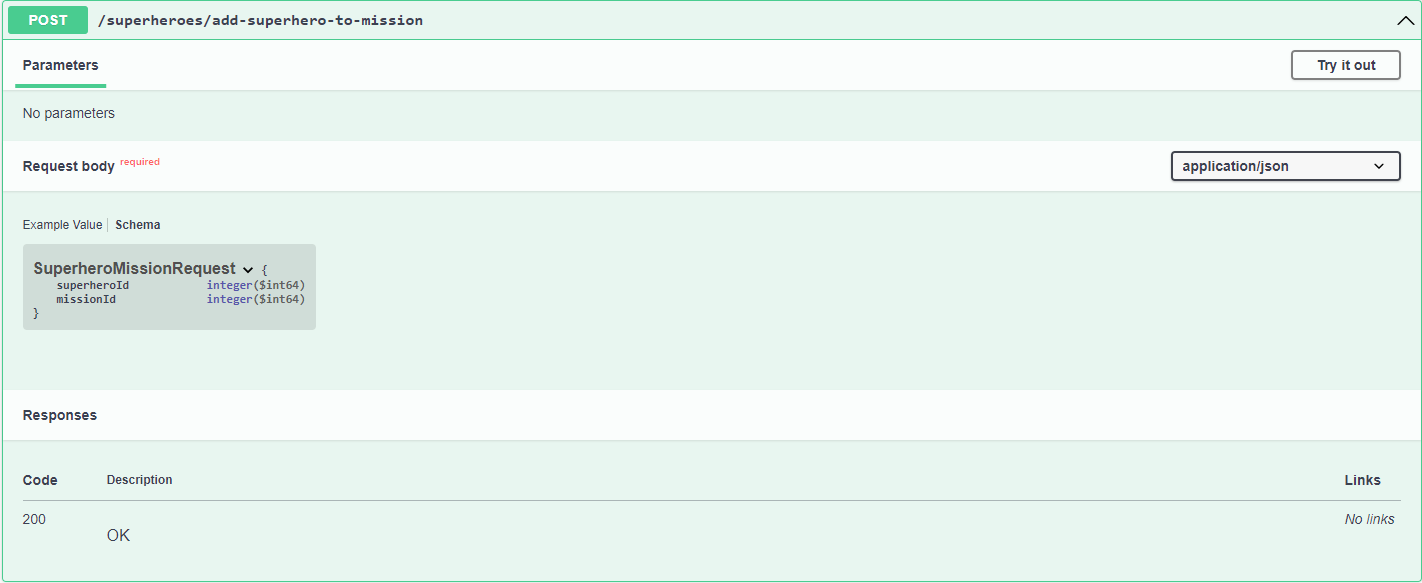
\includegraphics[width=\textwidth]{./images/chapter-jpa/superhero_controller_add_superhero_to_mission}

\begin{lstlisting}
package be.pxl.superhero.service.impl;

import be.pxl.superhero.api.SuperheroDTO;
import be.pxl.superhero.api.SuperheroRequest;
import be.pxl.superhero.domain.Mission;
import be.pxl.superhero.domain.Superhero;
import be.pxl.superhero.exception.ResourceNotFoundException;
import be.pxl.superhero.repository.MissionRepository;
import be.pxl.superhero.repository.SuperheroRepository;
import be.pxl.superhero.service.SuperheroService;
import org.springframework.stereotype.Service;
import org.springframework.transaction.annotation.Transactional;

import java.util.List;

@Service
public class SuperheroServiceImpl implements SuperheroService {

    private final SuperheroRepository superheroRepository;
    private final MissionRepository missionRepository;

    public SuperheroServiceImpl(SuperheroRepository superheroRepository,
                                MissionRepository missionRepository) {
        this.superheroRepository = superheroRepository;
        this.missionRepository = missionRepository;
    }

   
    // other methods not included 

    @Transactional
    public void addSuperheroToMission(Long superheroId, Long missionId) {
        Superhero superhero = superheroRepository.findById(superheroId).orElseThrow(() -> new ResourceNotFoundException("Superhero", "ID", superheroId));
        Mission mission = missionRepository.findById(missionId).orElseThrow(() -> new ResourceNotFoundException("Mission", "ID", missionId));
        superhero.addMission(mission);
    }
}
\end{lstlisting}

In the service-layer we retrieve our superhero and mission entity objects (and throw an exception if they don't exist). Then, the mission entity object is added to the superhero's mission and otherwise. Thanks to the @Transactional annotation, all this runs in one transaction. When the transaction is commited, the updated superhero entity is synchronized with the database and the changes are stored in the database. In other words, a record is saved in the link table when no exception occurs. If an exception occurs, the transaction is rolled back.


Lastly, we need DTO's with extra fields with the detailed superhero and mission information.

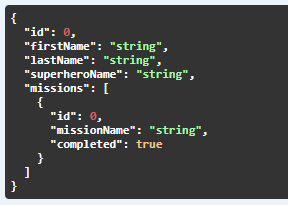
\includegraphics{./images/chapter-jpa/superhero_detail_dto}


Overview of spring data jpa annotations.

Entity Definition
@Entity: Specifies that a class is an entity and is mapped to a database table.

@Column: Specifies the mapped column for a persistent property or field.
@Id: Marks a field as a primary key.
@GeneratedValue: Specifies the strategy for generating primary key values.
@Embedded: Indicates a field should be treated as an embeddable type.
@Embeddable: Marks a class to be embedded within an entity.

Fetching Strategy
@Fetch: Specifies a custom fetching strategy for an association.
@LazyCollection: Specifies that a collection should be loaded lazily.
Miscellaneous
@Transient: Marks a field as not persistent.


@Enumerated: Specifies that a persistent property or field should be persisted as an enumerated type.
Repository Support
@Repository: Indicates that an annotated class is a repository, which is an abstraction of data access and storage.
@Query: Specifies a SQL or JPQL query directly on the repository method.
@Modifying: Indicates that a query method should be considered as modifying query (such as UPDATE, DELETE).
Transaction Management
@Transactional: Specifies that a method or class must be executed within a transaction.



